\subsection{Series Converter}

The series converter dynamics are given by:

\begin{align}
    \begin{aligned}
        v_s^{abc} &= R_{fs}i_{fs}^{abc} + L_{fs}\dfrac{d\,i_{fs}^{abc}}{dt} + v_{cs}^{abc} \\
        i_{fs}^{abc} &= C_{fs}\dfrac{d\,v_{cs}^{abc}}{dt} + i_g^{abc} \\
    \end{aligned}
\end{align}
where $v_s^{abc}$ is the series converter output voltage, $i_{fs}^{abc}$ is the series converter inductor current, $v_{cs}^{abc}$ is the series converter output capacitor voltage, and $i_g^{abc}$ is the grid current after the coupling transformer. The parameters $R_{fs}$, $L_{fs}$, and $C_{fs}$ are the series converter filter resistance, inductance, and capacitance respectively.

Leaving the states on the left side, and converting to $\alpha\beta$ coordinates, the series converter model is given by:

\begin{figure*}
    \centering
    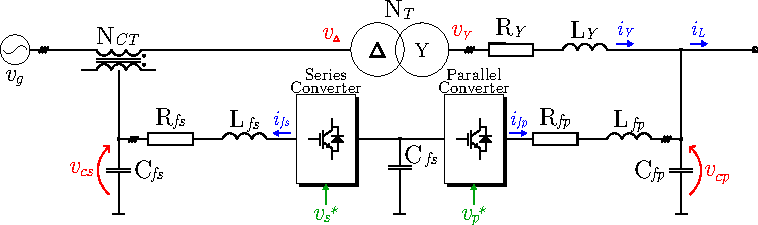
\includegraphics[width=0.9\textwidth]{Images/HDT_Diagram.pdf} 
    \caption{Hybrid distribution transformer circuit diagram.}
    \label{fig:HDT_Transformer}
\end{figure*}

\begin{align}
    \begin{aligned}
        \dfrac{d\,i_{fs}^{\alpha\beta}}{dt} &= -\dfrac{R_{fs}}{L_{fs}}i_{fs}{\alpha\beta} - \dfrac{1}{L_{fs}}v_{cs}{\alpha\beta} + \dfrac{1}{L_{fs}}v_s{\alpha\beta} \\
        \dfrac{d\,v_{cs}{\alpha\beta}}{dt} &= -\dfrac{1}{C_{fs}}i_{fs}{\alpha\beta} + \dfrac{1}{C_{fs}}i_g{\alpha\beta}
    \end{aligned}
\end{align}

\subsection{Parallel Converter}

The parallel converter dynamics are given by:

\begin{align}
    \begin{aligned}
        v_p^{abc} &= R_{fp}i_{fp}^{abc} + L_{fp}\dfrac{d\,i_{fp}^{abc}}{dt} + v_{cp}^{abc} \\
        i_{fp}^{abc} &= C_{fp}\dfrac{d\,v_{cp}^{abc}}{dt} - i_Y^{abc} + i_L^{abc}
    \end{aligned}
\end{align}
where $v_p^{abc}$ is the parallel converter output voltage, $i_{fp}^{abc}$ is the parallel converter inductor current, $v_{cp}^{abc}$ is the parallel converter output capacitor voltage, $i_Y^{abc}$ is the transformer $Y$ side current, and $i_L^{abc}$ is the load current. The parameters $R_{fp}$, $L_{fp}$, and $C_{fp}$ are the parallel converter filter resistance, inductance, and capacitance respectively.

Leaving the states on the left side, and converting to $\alpha\beta$ coordinates, the series converter model is given by:

\begin{align}
    \begin{aligned}
        \dfrac{d\,i_{fp}^{\alpha\beta}}{dt} &= -\dfrac{R_{fp}}{L_{fp}}i_{fp}^{\alpha\beta} - \dfrac{1}{L_{fp}}v_{cp}^{\alpha\beta} + \dfrac{1}{L_{fp}}v_p^{\alpha\beta} \\
        \dfrac{d\,v_{cp}^{\alpha\beta}}{dt} &= \dfrac{1}{C_{fp}}i_{fp}^{\alpha\beta} - \dfrac{1}{C_{fp}}i_Y^{\alpha\beta} + \dfrac{1}{C_{fp}}i_L^{\alpha\beta}
    \end{aligned}
\end{align}

\subsection{Distribution Transformer}

The transformer is connected in $\Delta-Y$ configuration, with the series converter (through the coupling transformer) connected to the $\Delta$ side, and the parallel converter connected to the $Y$ side. The $Y$ side has its neutral point grounded. The transformer equations are given by:

\begin{align}
    \begin{aligned}
        v_{Ya} &= N_{LFT}(v_{\Delta a} - v_{\Delta b}) \\
        v_{Yb} &= N_{LFT}(v_{\Delta b} - v_{\Delta c}) \\
        v_{Yc} &= N_{LFT}(v_{\Delta c} - v_{\Delta a})
    \end{aligned}
\end{align}
This can be expressed in matrix form as:
\begin{align}
    \begin{aligned}
        v_Y^{abc} &= N_{LFT}
        \underbrace{
        \begin{bmatrix}
            1 & -1 & 0 \\
            0 & 1 & -1 \\
            -1 & 0 & 1
        \end{bmatrix}
        }_{K_T'}
        v_{\Delta}^{abc}\\
        v_Y^{abc} &= N_{LFT} K_T' v_{\Delta}^{abc} \label{eq:Delta_Y_Transformation}
    \end{aligned}
\end{align}
In the other hand, the dynamics of the transformer are modeled as a series impedance referred to the $Y$ side. These transformer equations are given by:
\begin{align}
    v_{Y}^{abc} &= R_Yi_Y^{abc} + L_Y\dfrac{d\,i_Y^{abc}}{dt} + v_{cp}^{abc} \\
    \intertext{Assuming that there is no zero-sequence current, and using the expression given in \eqref{eq:Delta_Y_Transformation}, the transformer model can be expressed in $\alpha\beta$ coordinates as:}
    \dfrac{d\,i_Y^{\alpha\beta}}{dt} &= -\dfrac{R_Y}{L_Y}i_Y^{\alpha\beta} - \dfrac{1}{L_Y}v_{cp}^{\alpha\beta} + \dfrac{1}{L_Y}N_{LFT}K_T'v_{\Delta}^{\alpha\beta}
\end{align}

\subsection{Overall HDT Model}
The overall HDT model can be expressed in state-space form as:
\begin{align}
    \begin{aligned}
        \dfrac{d}{dt}
        \underbrace{
        \begin{bmatrix}
            x_s\\
            x_p
        \end{bmatrix}
        }_{x}
        &=
        \underbrace{
        \begin{bmatrix}
            \mathbf{A}_s & \mathbf{P}_{ig}\mathbf{M}_p \\
            \mathbf{P}_{vc}\mathbf{M}_s & \mathbf{A}_p
        \end{bmatrix}
        }_{\mathbf{A}}
        \underbrace{
        \begin{bmatrix}
            x_s\\
            x_p
        \end{bmatrix}
        }_{x}
        +
        \underbrace{
        \begin{bmatrix}
            \mathbf{B}_s & \mathbf{0} \\
            \mathbf{0} & \mathbf{B}_p
        \end{bmatrix}
        }_{\mathbf{B}}
        \underbrace{
        \begin{bmatrix}
            u_s\\
            u_p 
        \end{bmatrix}
        }_{u}
        \\
        &+
        \underbrace{
        \begin{bmatrix}
            \mathbf{0}\\
            \mathbf{P}_{vg}
        \end{bmatrix}
        }_{\mathbf{P}_{vg}}
        v_g
        +
        \underbrace{
        \begin{bmatrix}
            \mathbf{0}\\
            \mathbf{P}_{iL}
        \end{bmatrix}
        }_{\mathbf{P}_{iL}}
        i_L
    \end{aligned}
\end{align}
where the matrices $\mathbf{M}_p = \begin{bmatrix}\mathbf{0} & \mathbf{I} & \mathbf{0}\end{bmatrix}$ and $\mathbf{M}_s = \begin{bmatrix}\mathbf{0} & \mathbf{I}\end{bmatrix}$ are used to select the appropriate states from the parallel and series converter state vectors respectively.

The last can be expressed in a more compact form as:
\begin{align}
    \begin{aligned}
        \dfrac{d\, x(t)}{dt} &= \mathbf{A}x(t) + \mathbf{B}u(t) + \mathbf{P}_{vg}v_g(t) + \mathbf{P}_{iL}i_L(t)\\
        y(t) &= \mathbf{C}\,x(t)
    \end{aligned}
\end{align}
with the states $x(t) = \begin{bmatrix} i_{fs}^{\alpha\beta} & v_{cs}^{\alpha\beta} & i_{fp}^{\alpha\beta} & i_{Y}^{\alpha\beta} & v_{cp}^{\alpha\beta} \end{bmatrix}^T$, input $u(t) = \begin{bmatrix} v_s^{\alpha\beta} & v_p^{\alpha\beta} \end{bmatrix}^T$, and output \linebreak $y(t) = \begin{bmatrix} i_{fs}^{\alpha\beta} & v_{cs}^{\alpha\beta} & i_{fp}^{\alpha\beta} & i_{Y}^{\alpha\beta} & v_{cp}^{\alpha\beta} \end{bmatrix}^T$.

The HDT system is discretized using a zero-order hold with a sampling time of $T_s = 5\,\mu s$. The discrete-time state-space model is given by:
\begin{align}
    \begin{aligned}
        x[k+1] &= \mathbf{A}_d x[k] + \mathbf{B}_d u[k] + \mathbf{P}_{vg,d} v_g[k] + \mathbf{P}_{iL,d} i_L[k]\\
        y[k] &= \mathbf{C} x[k]
    \end{aligned}
\end{align}
where $\mathbf{A}_d = e^{\mathbf{A}T_s}$, $\mathbf{B}_d = \int_0^{T_s} e^{\mathbf{A}\tau} d\tau \mathbf{B}$, $\mathbf{P}_{vg,d} = \int_0^{T_s} e^{\mathbf{A}\tau} d\tau \mathbf{P}_{vg}$, $\mathbf{P}_{iL,d} = \int_0^{T_s} e^{\mathbf{A}\tau} d\tau \mathbf{P}_{iL}$, and $\mathbf{C} = \mathbb{I}$.

Since the HDT is designed to have a one-sampling period delay in the control loop, the discrete-time model can be expressed as:
\begin{align}
    \begin{aligned}
        x[k+1] &=
        \begin{bmatrix}
            \mathbf{A}_d & \mathbf{B}_d \\
            \mathbf{0} & \mathbf{0}
        \end{bmatrix}
        \begin{bmatrix}
            x[k]\\
            u[k-1]
        \end{bmatrix}
        +
        \begin{bmatrix}
            \mathbf{0}\\
            \mathbf{I}
        \end{bmatrix}
        u[k]
    \end{aligned}
\end{align}